\documentclass[12pt, openany]{book}
\usepackage[lmargin = 3cm, rmargin = 3cm, top=2cm]{geometry}
\usepackage{listings}
\usepackage{xcolor}
\usepackage[normalem]{ulem}
\usepackage{graphicx}
\usepackage{float}
\definecolor{warwickblue}{rgb}{0.0, 0.70, 0.87}
\definecolor{warwickorange}{rgb}{0.96, 0.48, 0.13}
\definecolor{warwickgold}{rgb}{0.53, 0.42, 0.07}
\definecolor{warwickred}{rgb}{0.54, 0.06, 0.17}
\definecolor{warwickgreen}{rgb}{0.47, 0.47, 0.02}

\definecolor{codegreen}{rgb}{0,0.6,0}
\definecolor{grey}{rgb}{0.9,0.9,0.9}
\definecolor{textgreen}{rgb}{0,0.6,0}
\definecolor{textpurple}{rgb}{0.36,0.19,0.41}
\definecolor{textblue}{rgb}{0.14, 0.34, 0.52}

\usepackage{footnote}



\usepackage{newfile}
\usepackage{currfile}
\newoutputstream{releasefixes}
\immediate\openoutputfile{\jobname.FixBeforeRelease}{releasefixes}

%text effects
\newcommand{\fbrtext}[1]{\textcolor{red}{\textbf{#1}}}

%text and file io
\newcommand{\fbr}[1]{\fbrtext{#1}\addtostream{releasefixes}{\currfilename: at Line \the\inputlineno : #1}}
 %% Sets up streams so you can flag things as \fbr{} and they will show in red and also appear in a custom file <filename>.FixBeforeRelease with line numbers to be fixed later

\newoutputstream{thingsyoumustdo}
\immediate\openoutputfile{\jobname.must}{thingsyoumustdo}

%Must-do text effects
\newcommand{\musttext}[1]{\textcolor{red}{\textbf{#1}}}

%Must  text and file io
\newcommand{\mustnt}[1]{\musttext{#1}\addtostream{thingsyoumustdo}{\noexpand\item #1}}
\newcommand{\must}[1]{\mustnt{#1}}
%% Sets up must, should, mustnt and shouldnt text extraction

\PassOptionsToPackage{hyphens}{url}\usepackage[colorlinks, linkcolor=warwickblue]{hyperref}

\usepackage[toc,section=section, seeautonumberlist]{glossaries}


%----------FILL IN HERE----------------------------
%Fill in title, subtitle, author names and typesetter for title page and pre-amble generation
\title{Document Title Here}
\author{CS Brady and H Ratcliffe}
%Ugly but it works...
\newcommand{\newsubtitle}{Subtitle}
\newcommand{\typesettername}{H Ratcliffe}
%-------DONE-----------------------------------------

%Make title and author available to title page
\makeatletter
\let\newtitle\@title
\let\newauthor\@author
\makeatother
\makesavenoteenv{table}


%Fortran and C specific parts are coloured
\newcommand{\fortonly}[1]{\textcolor{textblue}{#1}}
\newcommand{\conly}[1]{\textcolor{warwickred}{#1}}

%Presenter/typesetter notes. Defaults to swallowing, swap to other to leave unchanged
\newcommand{\presnote}[1]{}
%\newcommand{\presnote}[1]{#1}

\newcommand{\aside}[1]{\emph{#1}}

%Extra emphasis
\newcommand{\superemph}[1]{\textcolor{red}{\emph{#1}}}

%Shaded aside boxes
\usepackage[breakable]{tcolorbox}
\newenvironment{asidebox}[1]{
	\begin{tcolorbox}[width=0.95\textwidth,colback={grey}, breakable, title=#1]}
{\end{tcolorbox}   
}

\lstdefinelanguage{pseudo}
{
morekeywords={FUNCTION, MODULE, BEGIN, END, PRINT, FOR, DO, IF, ELSE, THEN, RETURN, ASSERT, AND, OR},
morekeywords=[2]{MAIN, INTEGER, ARRAY,REAL, FLAG, STRING},
morekeywords=[3]{OPENW, OPENR, CLOSE, WRITE},
sensitive=true,
morecomment=[l]{//}
}
%Dummy docs language to get nice formatting and colours easily
\lstdefinelanguage{docs}
{
morekeywords={int, char, const, double, class, flag},
morekeywords=[2]{Parameters, Returns},
sensitive=true,
morecomment=[l]{\#}
}
\lstdefinelanguage{make}
{
morekeywords={target},
morekeywords=[2]{prerequisites},
morekeywords=[3]{recipe},
sensitive=false,
morecomment=[l]{\#}
}
\lstdefinelanguage{debug}
{
morekeywords={break, print, run, continue, if, delete, clear, quit},
morekeywords=[2]{gdb},
sensitive=true,
morecomment=[l]{\#}
}


\lstdefinestyle{pseudostyle}{
    language=pseudo,
    tabsize=3,
    frame=shadowbox,
    rulesepcolor=\color{gray},
    commentstyle=\color{codegreen},
    keywordstyle=\color{textblue}\bf,
    keywordstyle=[2]\color{textpurple}\bf,
    keywordstyle=[3]\color{warwickred}\bf,
    stringstyle=\color{warwickred},
    numbers=left,
    numberstyle=\tiny,
    numbersep=5pt,
    breaklines=true,
    showstringspaces=false,
    basicstyle=\footnotesize
    %emph={str},emphstyle={\color{magenta}}
  } 
\lstdefinestyle{docstyle}{
    language=docs,
    tabsize=3,
    frame=shadowbox,
    rulesepcolor=\color{gray},
    commentstyle=\color{codegreen},
    keywordstyle=\color{textblue}\bf,
    keywordstyle=[2]\color{textpurple}\bf,
    keywordstyle=[3]\color{warwickred}\bf,
    stringstyle=\color{warwickred},
    numbers=left,
    numberstyle=\tiny,
    numbersep=5pt,
    breaklines=true,
    showstringspaces=false,
    basicstyle=\footnotesize
  } 
\lstdefinestyle{debugstyle}{
    language=debug,
    tabsize=3,
    frame=shadowbox,
    rulesepcolor=\color{gray},
    commentstyle=\color{codegreen},
    keywordstyle=\color{textblue}\bf,
    keywordstyle=[2]\color{textpurple}\bf,
    stringstyle=\color{warwickred},
    numbers=left,
    numberstyle=\tiny,
    numbersep=5pt,
    breaklines=true,
    showstringspaces=false,
    basicstyle=\footnotesize
    %emph={str},emphstyle={\color{magenta}}
  } 

\lstdefinestyle{makestyle}{
    language=make,
    tabsize=3,
    frame=shadowbox,
    rulesepcolor=\color{gray},
    commentstyle=\color{codegreen},
    keywordstyle=\color{textblue}\bf,
    keywordstyle=[2]\color{textpurple}\bf,
    keywordstyle=[3]\color{warwickred}\bf,
    stringstyle=\color{warwickred},
    numbers=left,
    numberstyle=\tiny,
    numbersep=5pt,
    breaklines=true,
    showstringspaces=false,
    basicstyle=\footnotesize
    %emph={str},emphstyle={\color{magenta}}
  } 

\lstdefinestyle{nostyle}{
    tabsize=3,
    frame=shadowbox,
    rulesepcolor=\color{gray},
    commentstyle=\color{codegreen},
    keywordstyle=\color{textblue}\bf,
    keywordstyle=[2]\color{textpurple}\bf,
    stringstyle=\color{warwickred},
    numbers=left,
    numberstyle=\tiny,
    numbersep=5pt,
    breaklines=true,
    showstringspaces=false,
    basicstyle=\footnotesize
  } 

\lstdefinestyle{pystyle}{
    language=python,
    tabsize=3,
    frame=shadowbox,
    rulesepcolor=\color{gray},
    commentstyle=\color{codegreen},
    keywordstyle=\color{textblue}\bf,
    stringstyle=\color{warwickred},
    numbers=left,
    numberstyle=\tiny,
    numbersep=5pt,
    breaklines=true,
    showstringspaces=false,
    basicstyle=\footnotesize
  } 
\lstdefinestyle{forstyle}{
    language=fortran,
    tabsize=3,
    frame=shadowbox,
    rulesepcolor=\color{gray},
    commentstyle=\color{codegreen},
    keywordstyle=\color{textblue}\bf,
    stringstyle=\color{warwickred},
    numbers=left,
    numberstyle=\tiny,
    numbersep=5pt,
    breaklines=true,
    showstringspaces=false,
    basicstyle=\footnotesize
  } 
\lstdefinestyle{cstyle}{
    language=c,
    tabsize=3,
    frame=shadowbox,
    rulesepcolor=\color{gray},
    commentstyle=\color{codegreen},
    keywordstyle=\color{textblue}\bf,
    stringstyle=\color{warwickred}\bf,
    numbers=left,
    numberstyle=\tiny,
    numbersep=5pt,
    breaklines=true,
    showstringspaces=false,
    basicstyle=\footnotesize
  } 
 %% Definitions for colours and code syntax highlighting

\makenoidxglossaries
\loadglsentries{glossary_defs}%% Your glossary words

\begin{document}
\begin{titlepage}
	\centering
	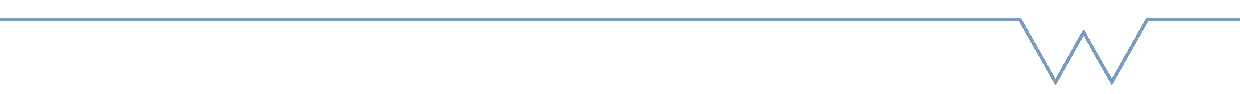
\includegraphics[width=0.95\textwidth]{Warwick_A4_Bar}\par\vspace{1cm}
	{\scshape\LARGE Warwick Research Software Engineering \par}
	\vspace{1cm}
	{\huge\bfseries \newtitle \par}
	{\large\bfseries \newsubtitle \par}
	\vspace{2cm}
	{\Large\itshape \newauthor \par}
	Senior Research Software Engineers\par
	\vspace{3cm}
	
\includegraphics[width=0.25\textwidth]{WarwickRSE}\par\vspace{1cm}
	{\scriptsize ``The Angry Penguin'', used under creative commons licence\\
from Swantje Hess and Jannis Pohlmann.}

	\vfill

% Bottom of the page
	{\large \today\par}
\end{titlepage} %% Fancy title page

\let\cleardoublepage\clearpage
\setcounter{tocdepth}{1}

\pagenumbering{gobble}
\tableofcontents


%% Boilerplate preamble
\frontmatter \chapter{Preface}
\section{About these Notes}
%----------FILL IN HERE----------------------------
These notes were written by \newauthor, Senior Research Software Engineers in the Scientific Computing Research Technology Platform at the University of Warwick for a Workshop first run in \fbr{When??} at the University of Warwick.
%----------DONE----------------------------

 %----------FILL IN HERE----------------------------
\textbf{This work, except where otherwise noted, is licensed under the Creative Commons Attribution-NonCommercial-NoDerivatives 4.0 International License. To view a copy of this license, visit \url{http://creativecommons.org/licenses/by-nc-nd/4.0/}}. 
\begin{figure}[h]
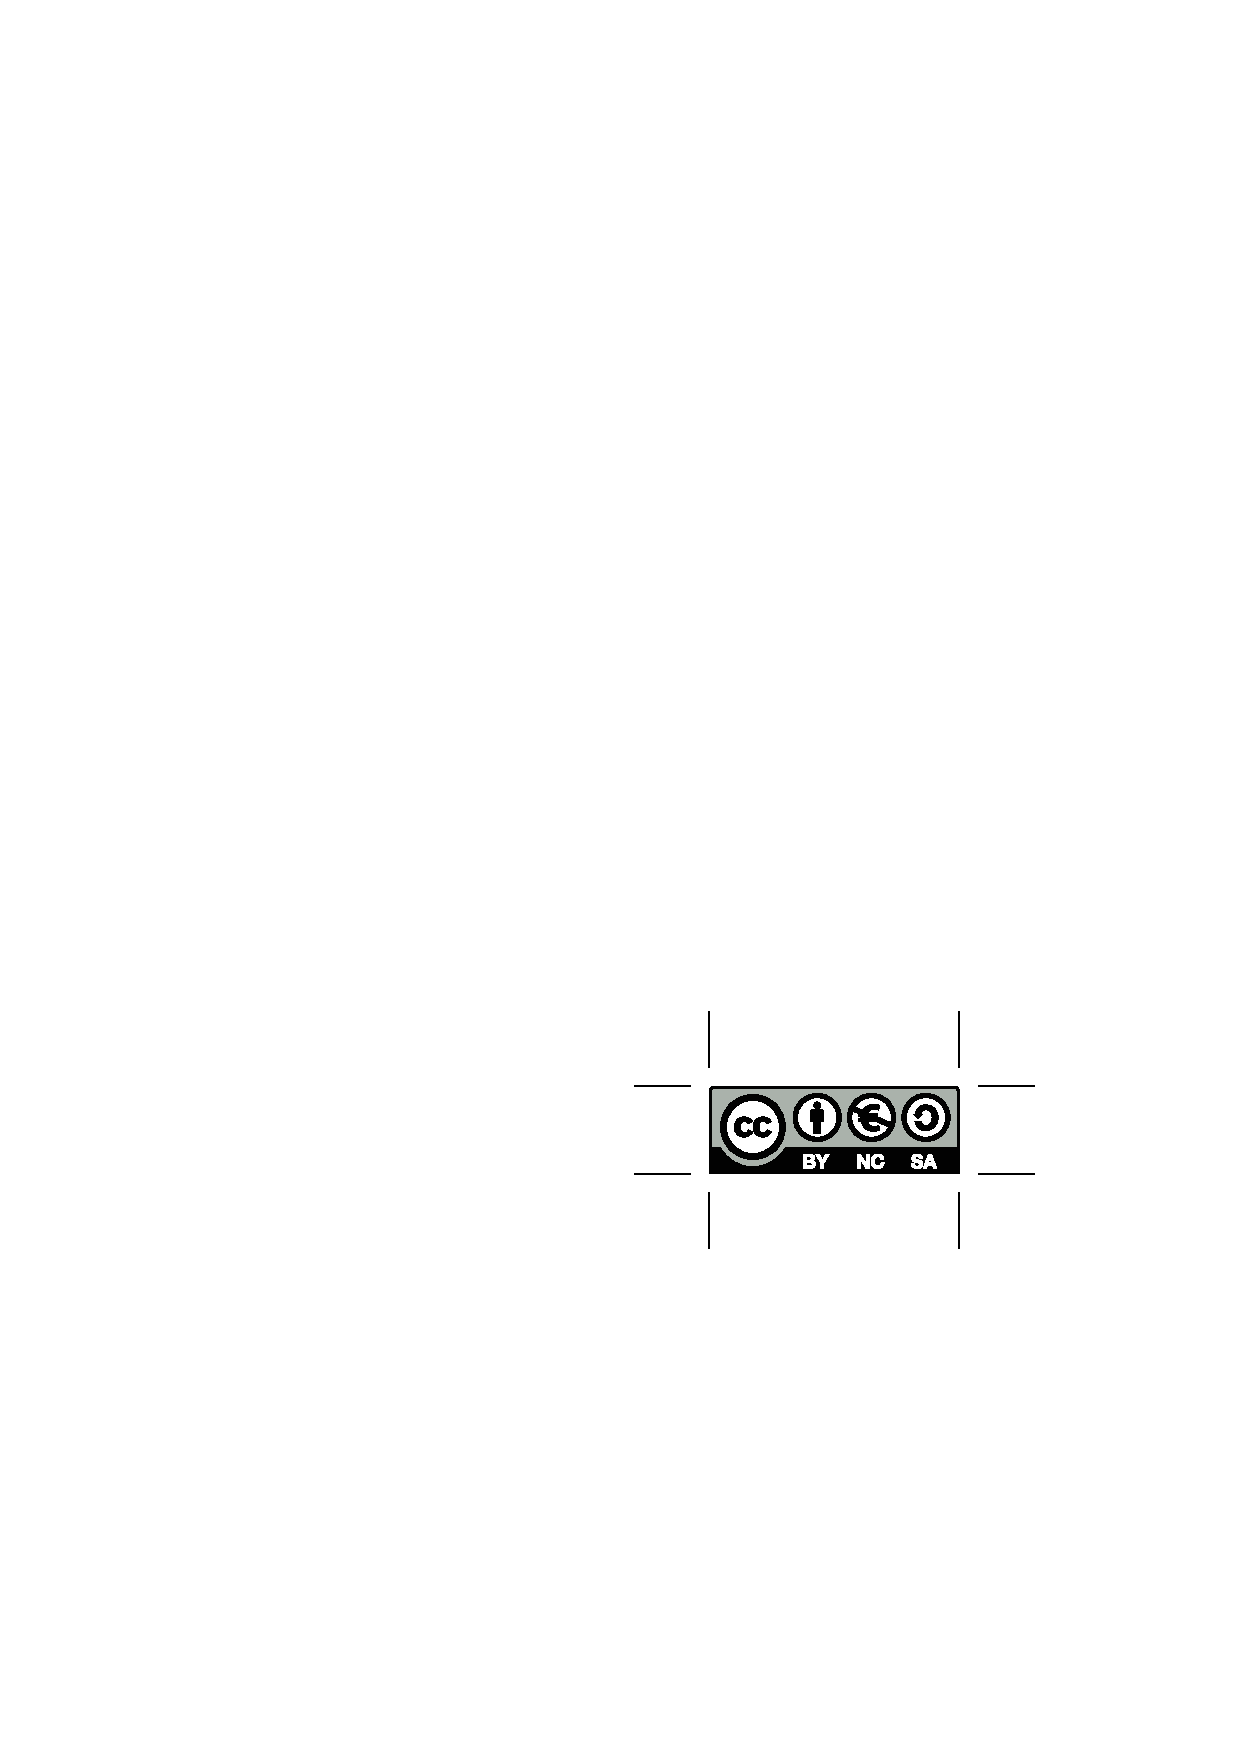
\includegraphics[width=0.15\textwidth]{by-nc-sa-eu}
\end{figure}

\noindent The notes may redistributed freely with attribution, but may not be used for commercial purposes nor altered or modified. The Angry Penguin and other reproduced material, is clearly marked in the text and is not included in this declaration. 
%----------DONE----------------------------

%% Name of typesetter!
The notes  were typeset in \LaTeX by \typesettername. \\Errors can be reported to \href{mailto:rse@warwick.ac.uk}{rse@warwick.ac.uk}

 %----------FILL IN HERE----------------------------
\section{Example Programs}\label{sec:egCode}
Several sections of these notes benefit from hands-on practise with the concepts and tools involved. Test code is available on Github at \url{https://github.com/WarwickRSE/}
%----------DONE----------------------------

\let\cleardoublepage\clearpage
\mainmatter
 %----------FILL IN HERE----------------------------
\chapter{Chapter Name}\label{chap:name}
\section{Section title}

\subsection{As usual...}

\textcolor{warwickgold}{\textbf{Some coloured text}}

\must{Here is a thing you must do} \mustnt{And A thing you must not}
\fbr{Do something here}
Text text tetx. \footnote{Footnote}
A \gls{processor} is a thing, its plural is \glspl{processor} An \gls{api} is a thing too

\begin{asidebox}{Box title}
Lorem Ipsum...
\end{asidebox}

Some code here
\begin{lstlisting}[style=pseudostyle]
variable item1 = 1;
variable item2 = 2;

\end{lstlisting}

\begin{lstlisting}[style=forstyle]
PROGRAM main
  INTEGER :: a
END PROGRAM
\end{lstlisting}

Inline code uses \lstinline{INTEGER} to get a similar styling

A figure. Should be configured to force them to appear right here, using the float package
\begin{figure}[h]
\center
\includegraphics[width=0.6\textwidth]{Images/tables}
\caption{Four tables with plates on}\label{fig:tables}
\end{figure}




%----------DONE----------------------------

\chapter{Glossary of Terms}
%Add all the glossary only terms
\printnoidxglossary

%%Close the streams so we can read from them below
\immediate\closeoutputstream{thingsyoumustdo}

%Optional - appendices
\appendix

%Include bullet lists of everything in must environment
\chapter{Golden Rules}\label{sec:thingsyoumustdo}
\section{Things You MUST ALWAYS do}
\begin{itemize}
    \input{\jobname.must}
\end{itemize}

 %Uncomment this to include Appendices containing all Must text

%Add all the glossary only terms (defined in glossary_defs but not used in text)
%Do this after all text etc, to get it right
\glsaddallunused 

\end{document}